% 
%	Jan Kechel
%	
%
\documentclass[landscape]{slides}
\usepackage{color,german}
\usepackage{graphicx}
%
\begin{document}
%
\title{TeamFound\\Infrastrukturen zur Open Source Softwareentwicklung\\Technische Universit"at Berlin}
\author{A. Bachmann, J. Heese, J. Kechel, M. Klink}
\date{WS 2005/2006}

%
\maketitle%
%
%%
\begin{slide}{Gliederung}

\textbf{1. Einf"uhrung}\\
Idee, Zielsetzung, Architektur-"Uberblick, Interface

\textbf{2. Implementation Server}\\
Architektur, Request/Response , Datenstruktur 

\textbf{3. Implementation Clients}\\
Web-Client, Firefox Toolbar, IE Toolbar

\textbf{4. Ablauf}\\
Beginn, 2005, 2006, Aktueller Stand

\textbf{5. Pr"asentation}
\end{slide}
%
%
%
%
\begin{slide}{1.1 Einf"uhrung}\\
TeamFound ist ..
\end{slide}
%
%
%
\begin{slide}{2.1 Architektur des Servers}\\
\begin{center}
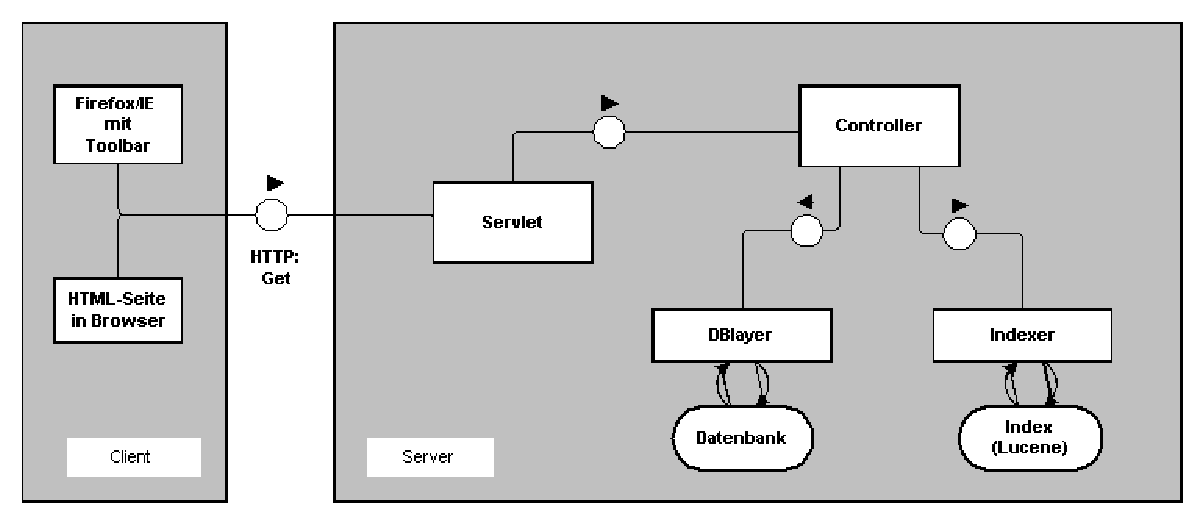
\includegraphics{bilder/aufbau2.eps}
\end{center}
\end{slide}
%
\begin{slide}{2.2 Request/Response }\\
\begin{itemize}
\item Anfrage-Parameter werden in Form von HTTP GET Variablen "ubertragen
\item Antworten vom Server
\begin{itemize}
\item HTML-Seite: die direkt im Browser angezeigt wird
\item XML-File: wird von der Toolbar interpretiert
\end{itemize}	
\end{itemize}
\end{slide}
%
\begin{slide}{2.2 Beispiel Request}\\
\begin{verbatim}
http://62.75.187.241:8080/tf/tf?keyword=teamfound
&want=xml&version=2&command=search&category=1
\end{verbatim}
\end{slide}
\begin{slide}{2.2 Beispiel Response }\\
\begin{verbatim}
<response>
	.
	.
	<search>	
		<result>
			<found>
				<url>http://teamfound.berlios.de</url>
				<title>TeamFound - share your search results</title>
				<incategory>0</incategory>
			</found>
		</result>
	</search>
</response>
\end{verbatim}
\end{slide}
%
\begin{slide}{2.3 Lucene Index}\\
\begin{itemize}
\item Wichtige Komponenten von Apache Lucene:
\begin{itemize}
\item Document und Field
\item Analyzer
\item Query
\end{itemize}
\end{itemize}
\end{slide}

%	
\begin{slide}{2.4 Datenstruktur}\\
\begin{center}
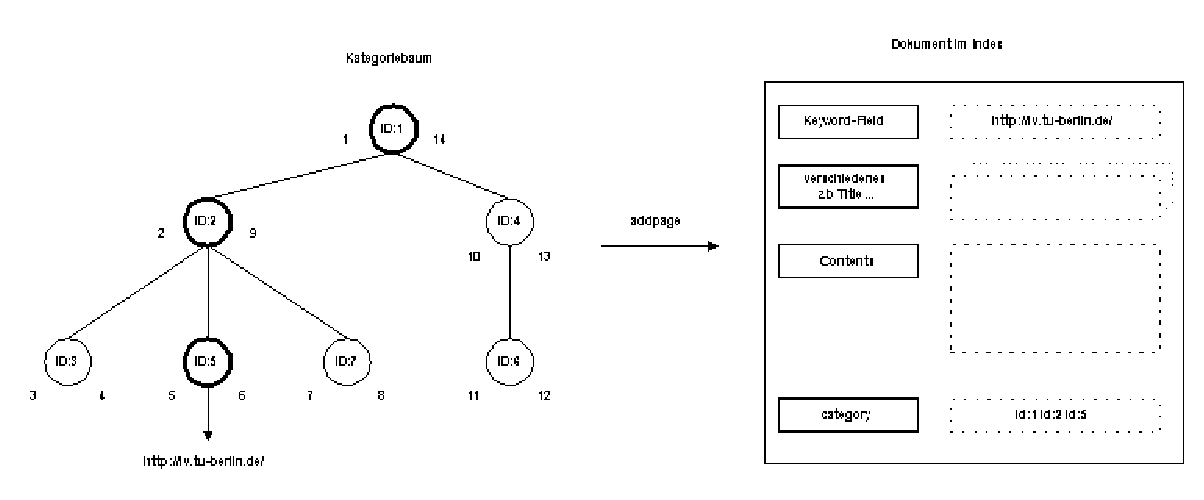
\includegraphics[width=17cm]{bilder/katstruktur.eps}
\end{center}
\end{slide}
%
%
%
\begin{slide}{3.1 Web-Client}\\

Web-Client ..

\end{slide}
%
\begin{slide}{3.2 Firefox Toolbar}\\
FF-Toolbar ..
\end{slide}
%
%
%
\begin{slide}{3.3 Internet Explorer Toolbar}\\
IE Toolbar ..
\end{slide}
%%
%%
%
\begin{slide}{4.1 Projektverlauf}\\
Das Projekt hat damit begonnen, ..
\end{slide}
%
%
%
\begin{slide}{5.1 Pr"asentation}\\
Pr"asentation
\end{slide}
%
%
%
%
\begin{slide}{}
The End
\end{slide}
%%%%%%%%%%%%%%%%%%%%%%%
\end{document}
